\chapter{Selected Gamification Features for English Mind}

Through systematic analysis of existing language learning applications and their gamification implementations, this chapter presents a carefully curated selection of gamification features for English Mind. 

The selection methodology prioritized features that have demonstrated effectiveness in existing applications while maintaining strong alignment with English Mind's core pedagogical principles. Identified features strategically enhance two critical aspects of the learning experience:

\begin{enumerate}
    \item \textbf{Enhanced Practice Experience} 
    \begin{itemize}
        \item Diversified flashcard types
        \begin{itemize}
            \item Word spelling
            \item Word pronunciation
            \item Word-Definition matching
            \item Word-Translation matching
        \end{itemize}
        \item Post-practice review providing immediate feedback and reinforcement
        \item Individual word progress tracking breaking the abstract concept of SRS into tangible stages
    \end{itemize}
    
    \item \textbf{Consistent Practice Motivation} 
    \begin{itemize}
        \item A streak system requiring daily engagement with new vocabulary
    \end{itemize}
\end{enumerate}

\newpage
\section{Diversified Flashcard Types}

The current English Mind's flashcard system employs a single format where users view an English word and recall its meaning. While effective for basic vocabulary acquisition, comparative analysis of language learning applications reveals that the monotony of a single flashcard type can reduce practice effectiveness. The variety in practice formats aims to maintain user interest throughout longer practice sessions, potentially increasing both practice duration and frequency.

This section proposes an expanded word revision system with five distinct flashcard types (see Figure \ref{fig:em-prototype-flashcard-types}), each targeting specific learning objectives.

\begin{enumerate}
    \item \textbf{Recall Meaning}

    The existing English Mind flashcard format, where users see an English word and recall its meaning, will be maintained as the foundation of the practice system. This format effectively tests basic word recognition and meaning recall (see Section \ref{sec:em-active-recall}).

    \item \textbf{Match Words to Translations}
    
    Following successful implementations in applications like Duolingo and WordUp, users match English words with their corresponding translations, presented in sets of five pairs. This format reinforces the connection between words in the target and native languages.

    \item \textbf{Match Words to Definitions}
    
    Similar to the translation matching, this format requires users to match English words with their definitions, reinforcing deeper understanding of word meanings. This format focuses on comprehension rather than translation.

    \item \textbf{Spell Word}
    
    This exercise type presents users with a word's definition and a contextual sentence containing a blank space. Users must correctly spell the target word to complete the sentence. An audio pronunciation button is available as a hint if users cannot determine the required word. The system evaluates spelling accuracy and provides immediate feedback.

    \item \textbf{Pronounce Word}

    Users are shown an English word and prompted to pronounce it correctly. The system evaluates pronunciation accuracy using speech recognition technology, providing binary feedback (correct/incorrect). Understanding that not all practice environments are suitable for speaking exercises, users can opt to skip these cards when needed.

\end{enumerate}
\newpage
\begin{figure}[!h]
    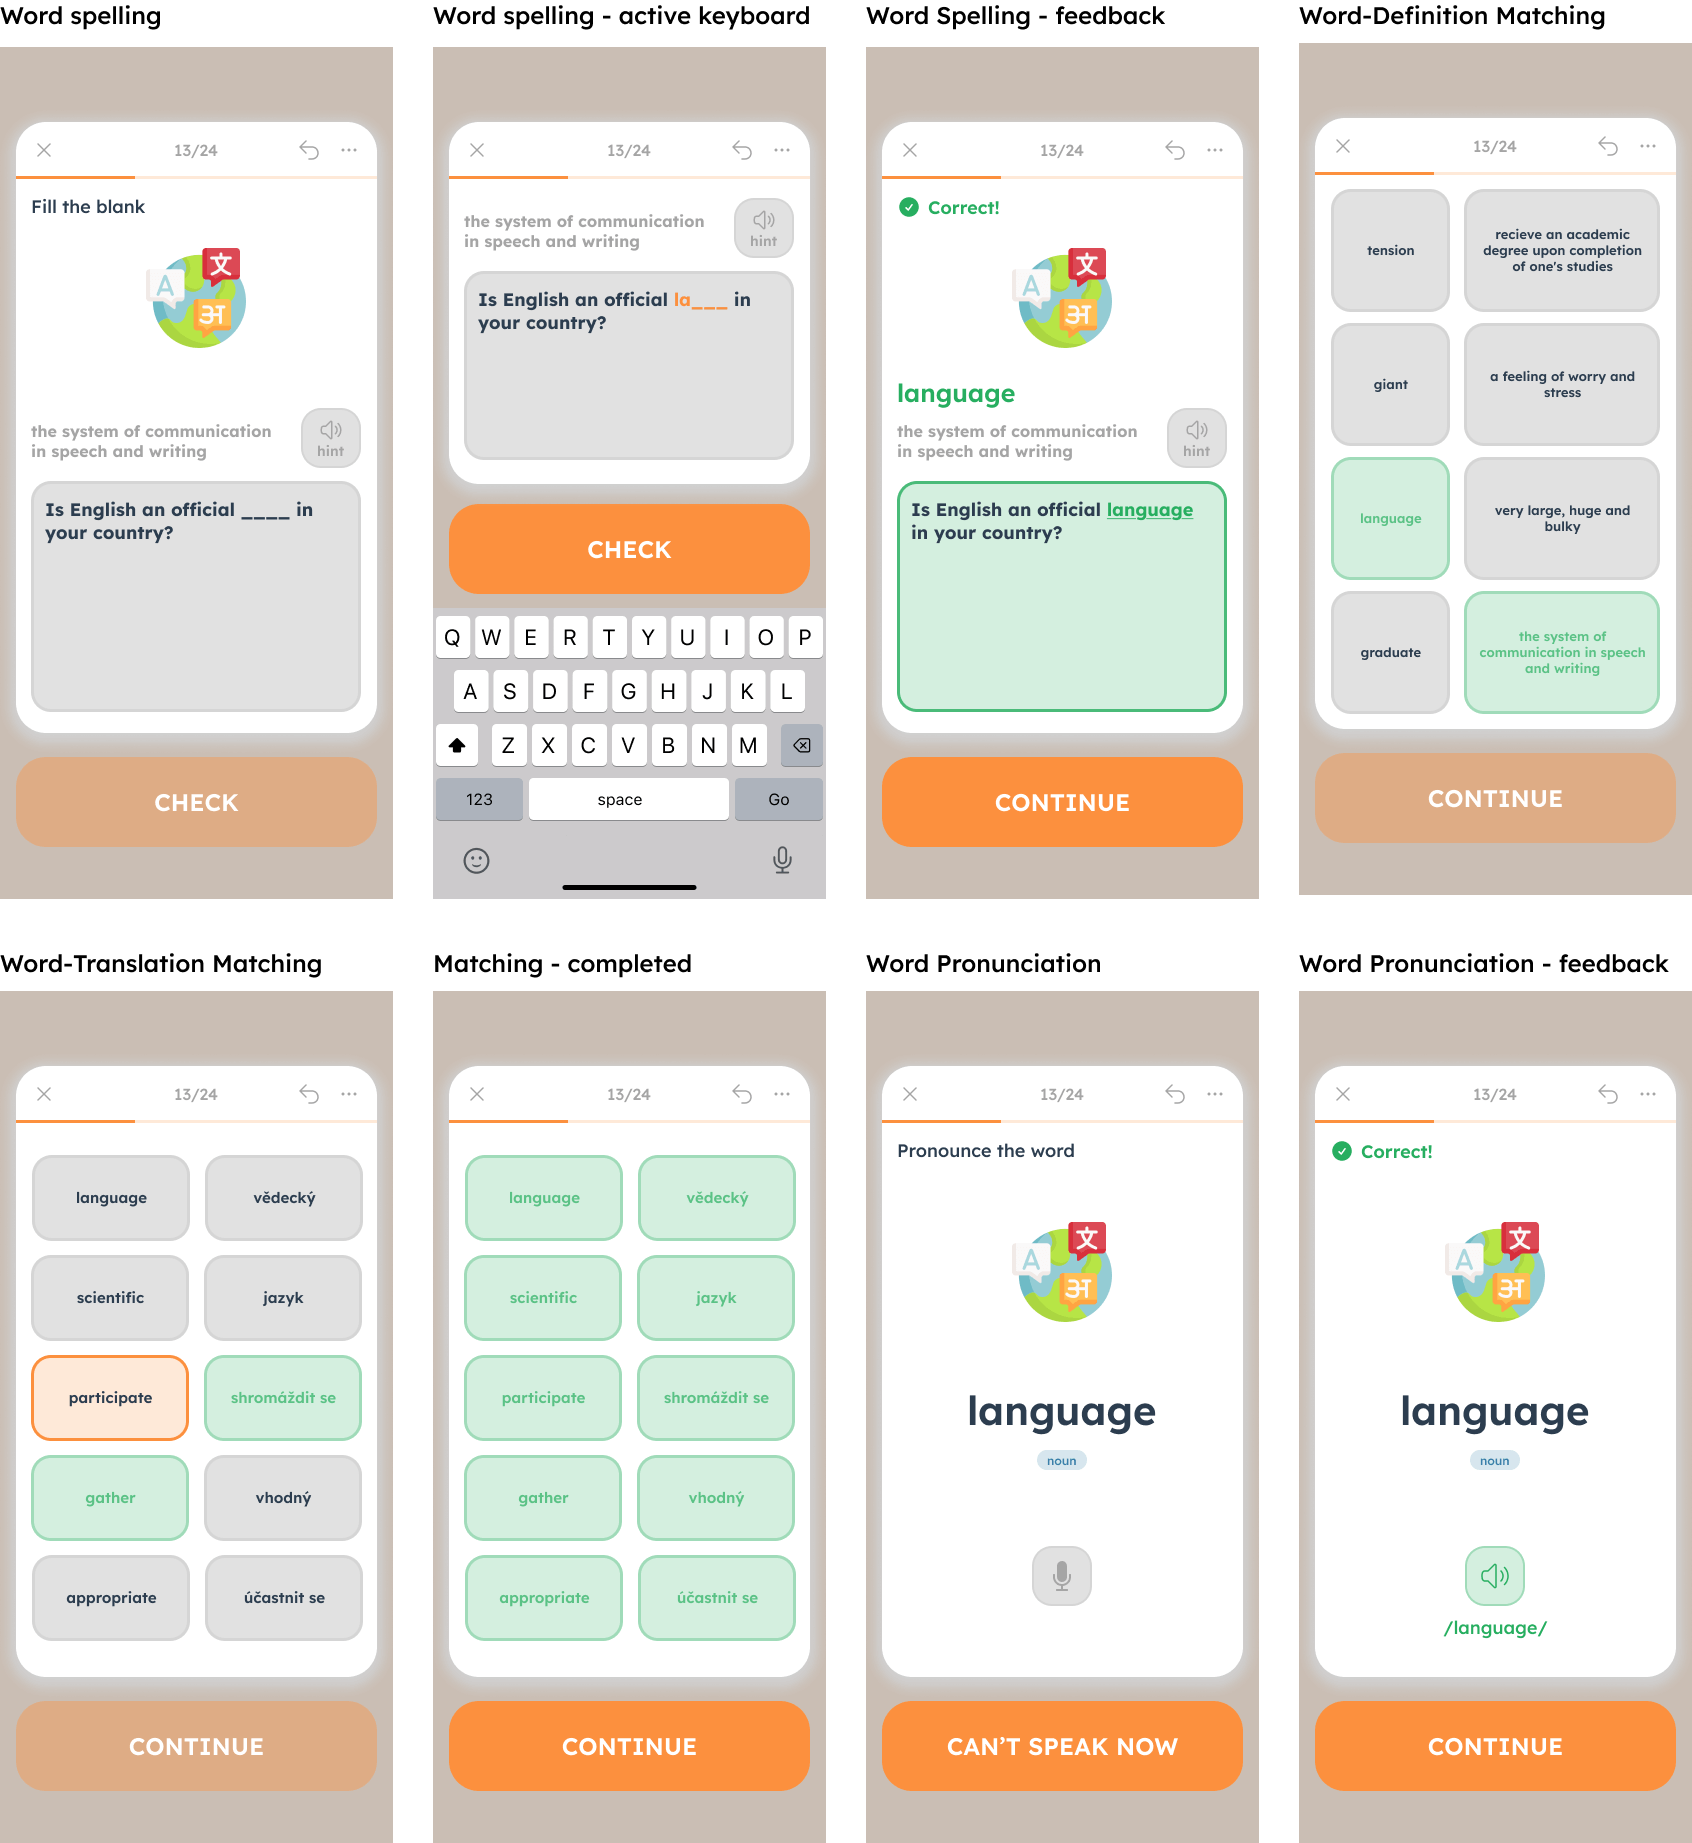
\includegraphics[width=1\textwidth]{src/figures/em-prototype-flashcards.png}
    \caption{Prototype - Flashcard Types}
    \label{fig:em-prototype-flashcard-types}
\end{figure}

The integration of new flashcard types requires careful consideration of the existing spaced repetition system. Only recall meaning flashcards will influence the SRS scheduling of words, while additional types (match, spell, and pronounce) serve as supplementary practice. This approach preserves the proven effectiveness of the current SRS algorithm while enhancing learning through varied practice formats.

The distribution of flashcard types in a practice session follows a structured approach. Recall meaning flashcards appear first and supplementary types follow in randomized order. This prioritization ensures that the core SRS algorithm remains the primary driver of vocabulary acquisition and prevents other flashcard types from inadvertently reminding users of word meanings before they attempt recall.

\section{Vocabulary Progress Tracking}

Inspired by WordUp's individual word progress tracking (see Section \ref{sec:wordup-individual-word-progress-experience}), we propose implementing a visual progress indicator system that integrates seamlessly with English Mind's existing spaced repetition system. This feature provides users with clear, immediate feedback on their progress with each vocabulary item, helping them understand where they stand in the learning journey for specific words. The visual indicator system maps the existing spaced repetition intervals into five distinct stages (see Table \ref{tab:vocabulary-progress-tracking-stages}).
\begin{table}[h]
    \centering
    \begin{tabular}{|c|l|l|}
        \hline
        \textbf{Stage} & \textbf{Name} & \textbf{SRS Interval} \\
        \hline
        1 & Starting & 0 minutes - 3 days \\
        \hline
        2 & Recognizing & 3 days - 1 week \\
        \hline
        3 & Reinforcing & 1 week - 3 weeks \\
        \hline
        4 & Strengthening & 3 weeks - 3 months \\
        \hline
        5 & Mastering & 3 months - 8 months \\
        \hline
    \end{tabular}
    \caption{Vocabulary Progress Tracking Stages}
    \label{tab:vocabulary-progress-tracking-stages}
\end{table}

The progress indicator appears only on the recall meaning flashcards (see Figure \ref{fig:em-prototype-word-progress}). It consists of five sequential boxes that fill progressively as the word advances through the stages, making the abstract concept of spaced repetition more concrete and understandable. The visual representation of progress creates a game-like element that enhances motivation and engagement.

\begin{figure}[!h]
    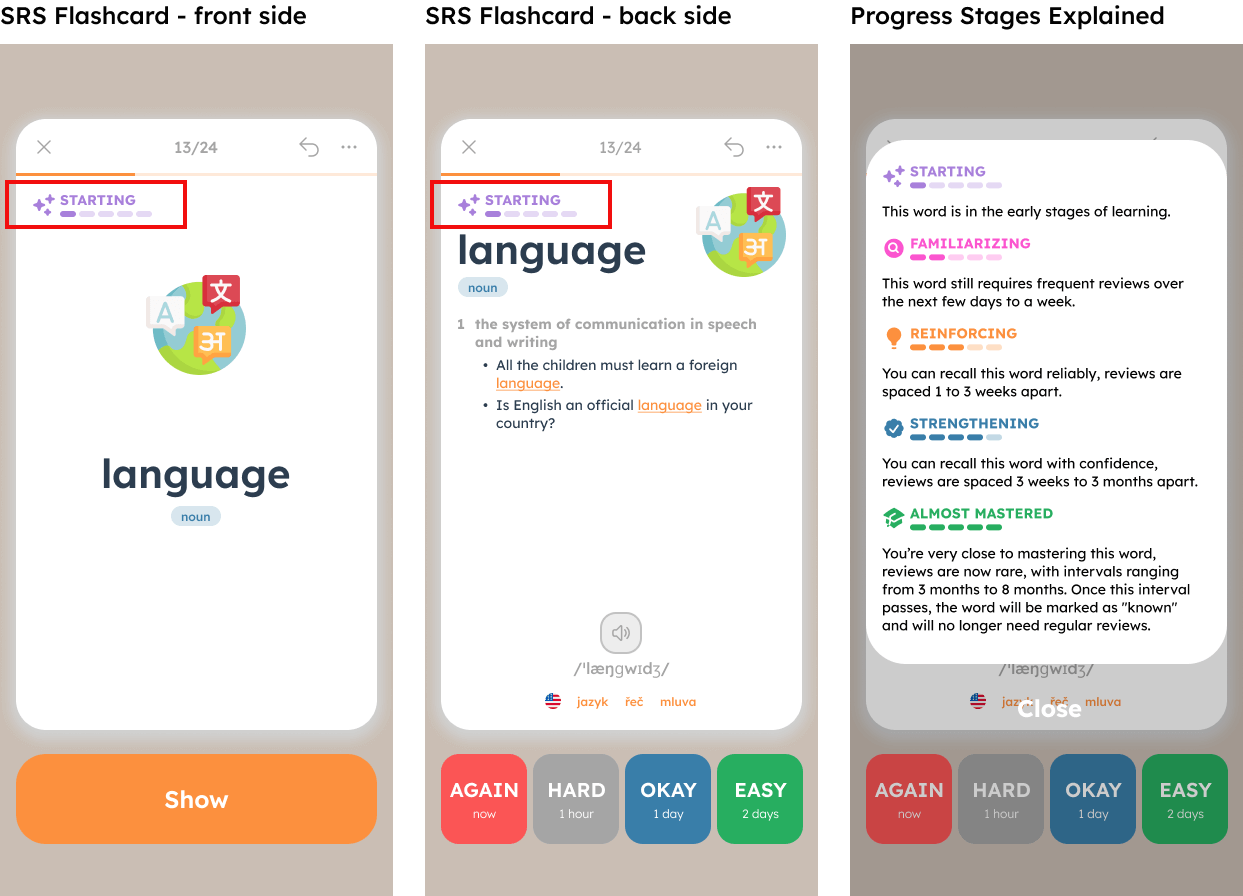
\includegraphics[width=0.86\textwidth]{src/figures/em-prototype-progress-system.png}
    \caption{Prototype - Vocabulary Progress Tracker}
    \label{fig:em-prototype-word-progress}
\end{figure}

\section{Post-Practice Review}

The post-practice review screen provides immediate feedback after completing a practice session (see Figure \ref{fig:em-prototype-practice-review}). It displays key metrics including the number of words practiced and time spent, accompanied by a brief motivational message. The implementation includes a lightweight confetti animation to provide positive reinforcement for session completion. This feature aims to increase user engagement and potentially increase practice session completion rates.
\begin{figure}[!h]
    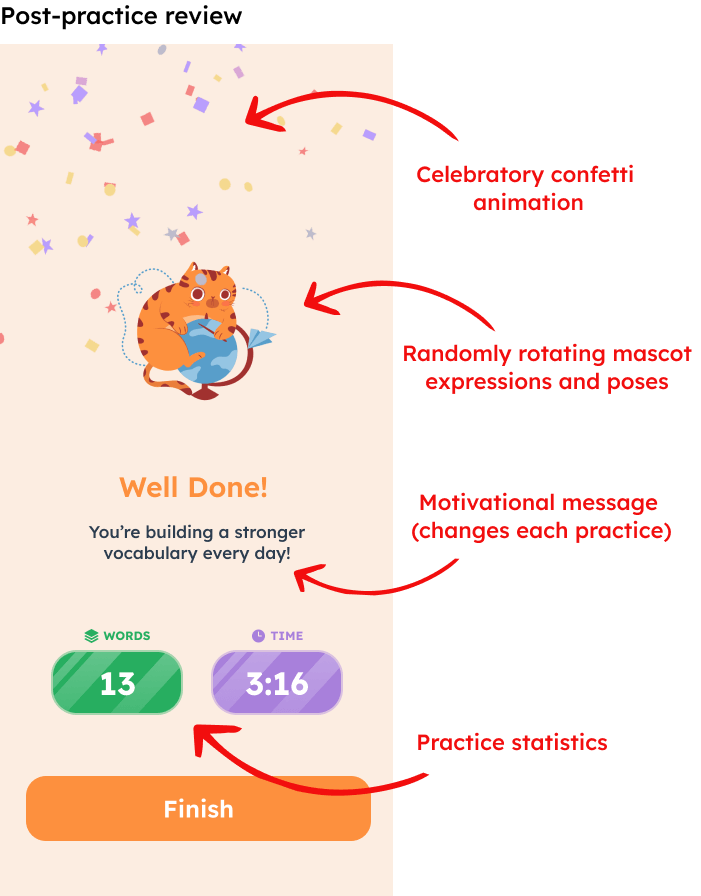
\includegraphics[width=0.8\textwidth]{src/figures/em-prototype-review.png}
    \caption{Prototype - Post-Practice Review}
    \label{fig:em-prototype-practice-review}
\end{figure}

\section{Streak System}

The streak system draws inspiration from successful implementations in language learning applications like Duolingo, where 20\% of 
daily active users maintain streaks exceeding one year \cite
{cite:duolingo_2024q2}. The system implements a daily engagement mechanism that requires users to learn at least one new vocabulary item per day to maintain their active streak. This design choice balances the need for consistent progress with manageable daily commitments. It provides users with a clear, quantifiable metric for tracking their consistency. This approach facilitates the development and maintenance of regular practice habits.

The system deliberately omits advanced features such as streak freezes or recovery options, prioritizing the establishment and validation of core streak mechanics. This simplified approach allows for future feature expansion based on empirical user engagement data and feedback.

The system's visual implementation comprises two distinct components. The primary interface element is the streak counter (badge), prominently displayed at the top of the main screen (see Figure \ref{fig:em-prototype-streak}). This counter features a numerical representation of consecutive practice days, employing distinct visual states to indicate streak status: a golden appearance for active streaks and a faded state when the streak is at risk.

The second component focuses on achievement recognition. Upon successful completion of daily practice, a celebration screen appears displaying the updated streak count and a weekly progress visualization. The weekly view presents the current week's practice activity (Monday through Sunday), with perfect weeks highlighted in a special golden frame to recognize consistent engagement.

\begin{figure}[!h]
    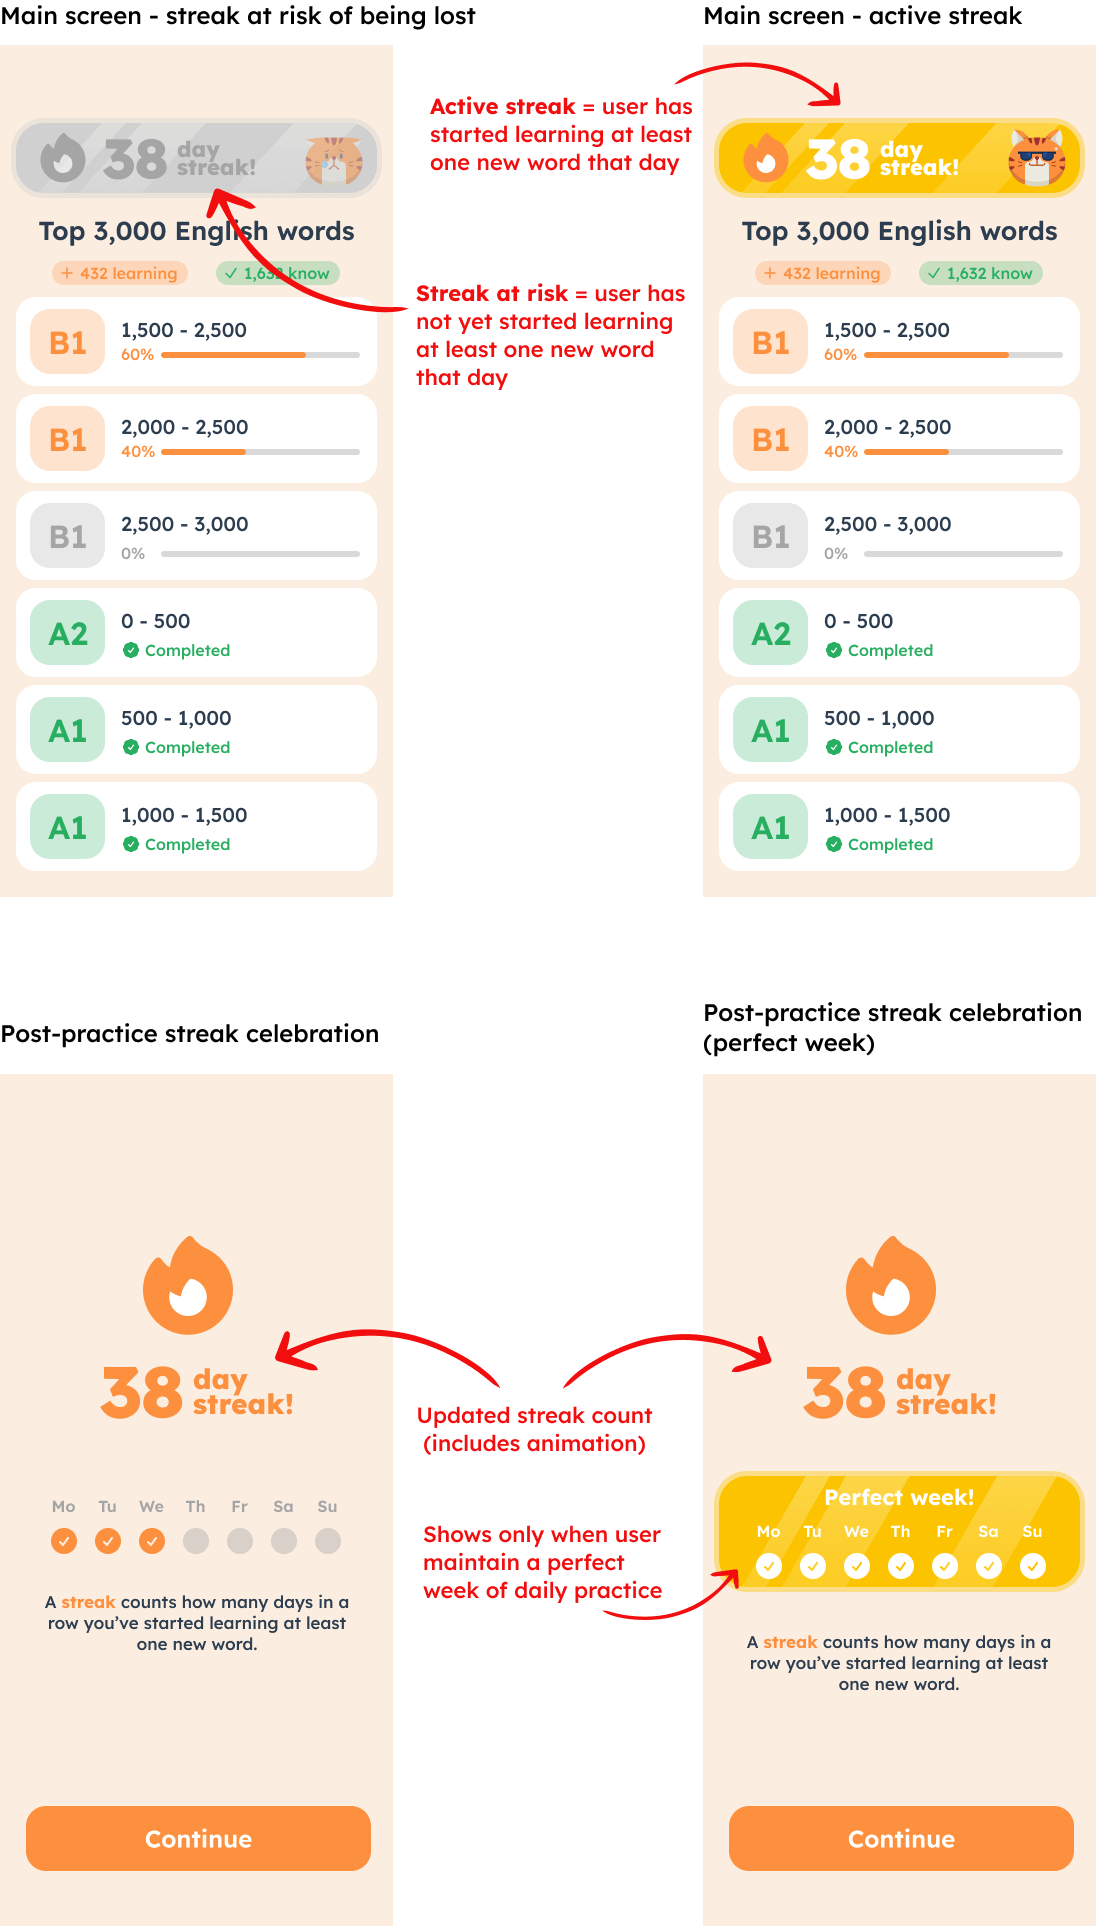
\includegraphics[width=0.88\textwidth]{src/figures/em-prototype-streak.png}
    \caption{English Mind - Prototype: Streak Implementation}
    \label{fig:em-prototype-streak}
\end{figure}